\documentclass[10pt, conference, compsocconf]{IEEEtran}
\usepackage{tabularx} % extra features for tabular environment
\usepackage{amsmath}  % improve math presentation
\usepackage{graphicx} % takes care of graphic including machinery
\usepackage{algorithm}% http://ctan.org/pkg/algorithms
\usepackage{algpseudocode}% http://ctan.org/pkg/algorithmicx
\usepackage{caption}
\usepackage{subcaption}
\usepackage{color}
%% \usepackage{minted}
\usepackage[margin=1in,letterpaper]{geometry} % decreases margins
\usepackage{cite} % takes care of citations
%% \usepackage[final]{hyperref} % adds hyper links inside the generated pdf file
%% \hypersetup{
%% 	colorlinks=true,       % false: boxed links; true: colored links 
%% 	linkcolor=blue,        % color of internal links
%% 	citecolor=blue,        % color of links to bibliography 
%% 	filecolor=magenta,     % color of file links 
%% 	urlcolor=blue          
%% }  

%% \lstset{  
%%   frame=none,    
%%   xleftmargin=2pt,
%%   stepnumber=1, 
%%   numbers=left,
%%   numbersep=5pt,
%%   numberstyle=\ttfamily\tiny\color[gray]{0.3},
%%   belowcaptionskip=\bigskipamount,
%%   captionpos=b,
%%   escapeinside={*'}{'*},
%%   language=haskell,  
%%   tabsize=2,
%%   emphstyle={\bf},
%%   commentstyle=\it,
%%   stringstyle=\mdseries\rmfamily, 
%%   showspaces=false,
%%   keywordstyle=\bfseries\rmfamily,
%%   columns=flexible,
%%   basicstyle=\small\ttfamily, %sffamily,
%%   showstringspaces=false,
%%   morecomment=[l]\%,
%% }

%\usepackage[noadjust]{cite}

\begin{document}  
\title{Optimizing Cloud-Based Networks for Lower Latency Using Learned Machine Characteristics}
 
\author{\IEEEauthorblockN{John L. Singleton}
  \IEEEauthorblockA{Department of Computer Science\\
    University of Central Florida\\
    Orlando, Florida 32816\\
    Email: jls@cs.ucf.edu}
\and
\IEEEauthorblockN{Mohammad Ahmadian}
\IEEEauthorblockA{Department of Computer Science\\
    University of Central Florida\\
    Orlando, Florida 32816\\
    Email: ahmadian@cs.ucf.edu}
\and
\IEEEauthorblockN{Gary T. Leavens}
\IEEEauthorblockA{Department of Computer Science\\
    University of Central Florida\\
    Orlando, Florida 32816\\
    Email: leavens@cs.ucf.edu}
}

\maketitle

\begin{abstract}
Cloud Service Providers allocate machine instances non-contiguously to achieve higher utilization of their resources. This allocation method makes it difficult to control the network latency between instances. Latency is a key bottleneck for many computational workloads, especially those found in scientific and big data tasks. In this paper, we propose a novel method for extracting latency-optimal clusters within a non-contiguously allocated machine instance environment. We provide an evaluation of the effectiveness of our method in the context of optimizing a large computing cluster on Amazon Web Services. 
\end{abstract}

\begin{IEEEkeywords}
Cloud computing, latency, Machine learning, Amazon Web Services, Data-Driven, Cluster
\end{IEEEkeywords}

\section{Introduction and Motivation} \label{sec:introduction}
\begin{figure*}[ht] 
  \centering
  \includegraphics[scale=.4]{figures/big-plot-edited.pdf}
  \caption{Latency by Clique found in our initial experiment. Note that as the Clique size increases, the likelyhood that the average latency will be higher grows. We see the lowest latencies in a clique of size 2. For reference, we show the theoretical latencies of InfiniBand and GigE networks.}
  \label{fig:clique}
\end{figure*}

Latency is an important aspect of computer networks that can impact the performance of applications. Because of this, many large super computers such as Lawrencium (at UC Berkeley) and Franklin (at the Department of Energy) take into consideration the task minimizing latency in their interconnection networks.

One of the most recent trends in computing and that of \textit{Cloud Computing}. One of the primary advantages of cloud computing approaches is that of low cost and flexibility. The configuration of cloud computing resources is typically performed via software API calls. While super computers are the dominant form of high performance computing in terms of performance, increasing access to Cloud Computing resources offers an opportunity---if a sufficiently powerful computing cluster can be created from the available computing resources. 

In 2010, Jackson et al conducted a study examining the performance of Amazon EC2 relative to two traditional super computers. In their results the researchers observed that the performance of EC2 was as much as 2-20 times worse than the traditional super computers, and that one of the major contributing factors was the latency of the Amazon network \cite{jackson_performance_2010}.

However, latency isn't the only factor complicating the goal of using EC2 for super computing tasks. Jackson et al. writes:

\begin{quote}
  ``Amazon offers no guarantees on proximity of nodes allocated together, and there is significant variability in latency between nodes."
  \end{quote}

Further complicating matters, Jackson et al. observes:  

\begin{quote}
  ``In addition to the variability in network latency, we also see variability in the underlying hardware the virtual machines are running on. By examining /proc/cpuinfo we are able to identify the actual CPU type of the un-virtualized hardware."
\end{quote}


Because when users request new servers on cloud computing networks they have no control over the placement of the server (relative to other servers) the latency of networks built in the cloud are unpredictable. This fact makes it difficult to build high performance computer clusters in the cloud. 

The rest of this paper is organized as follows: In Section \ref{sec:feasibility}, we discuss the limitations naively attempting to find an optimal network. In Section \ref{sec:experimental} we detail the experiments we performed to evaluate the effectiveness of optimizing a test network with three different methods. We contrast a naive, greedy, and machine learning approach.  The result of all three approaches and discussion are presented in Section \ref{sec:results}. Finally, in Section \ref{sec:conclusion} we summarize the results of this study.      
    
\section{Creating Optimal Networks in the Cloud}

There is one important difference between the interconnection networks used in the Cloud versus those used in super computers. Namely, while cloud networks use some form of Ethernet connectivity, high-performance super computers typically use high speed interconnects such as InfiniBand, which have far less latency than Ethernet. This difference can be between 12 and 100 times slower, with InfiniBand having latency in the 1$\mu s$ range. In Table \ref{table:latencies} we list some of the latencies of common interconnection technologies.

\begin{table}[h]
\centering
\caption{Typical latency of various network connection technologies.}
\begin{tabular}{| c | c |}
\hline
Technology  & Latency ($\mu s$) \\
\hline
\hline
GigE & 29-100 \\
\hline 
10 GigE & 21.51 \\
\hline 
DDR InfiniBand  & 1.72 \\
\hline 
QDR InfiniBand & 1.67 \\
\hline 
\end{tabular}
\label{table:latencies}
\end{table}

In our work, we propose the idea that deploying an application to a cloud network is essentially a runtime problem of the following formulation:

\begin{quote}
\textit{Given a target topology $T$ and a specification $S$, find the optimal subgraph $s$ of the network $N$, such that $s$ satisfies $S$ with respect to $T$}
\end{quote}

In this paper we consider the topology of a network ($T$) to be expressed by the connectivity between nodes. That is, in a computational cluster, which nodes must communicate with to which nodes. For simplicity, in this paper all communication requirements are assumed to be bi-directional. We consider the latency requirements of a network to be analogous to its specification ($S$), e.g., \textit{no link between two nodes may have more than 5 ms in latency}. In our formulation, we form topologies by finding a smaller, optimal network ($s$) within larger group of candidate nodes ($N$). In the following sections we will describe this problem and our approach to solving it. 
\section{Feasibility of Approach} \label{sec:feasibility}

In an attempt to gain an understanding of the limitations of Cloud networks, we performed an initial experiment analyzing the performance of randomly formed cloud networks.

To determine this we initialized 100 EC2 micro instances and computed a fixed topology of sizes ranging from $N=2$ to $N=5$. The networks computed are the \textit{complete subgraph} of the network. Such a network is commonly known as a \textit{Clique} \cite{Sipser:2012ta}. In this topology, each pair of nodes is adjacent to one another. As mentioned in \ref{sec:introduction}, we assume for any pair of connected nodes that the communication is bidirectional.  

A related problem is the \textit{maximum clique} problem  which aims to find the largest subset of vertices such that every two nodes are connected by an edge. The brute force search algorithms iteratively inspect all subsets to identify the maximum clique (largest clique by vertices) in the graph of that models the problem. Unfortunately, this problem is one of the NP-complete problems and it may require exponential time.

To setup our initial experiment we considered all the possible networks with the Clique topology that could be formed of sizes ranging from $N=2$ to $N=5$ from a network with 100 nodes. Because many networks can be formed from 100 nodes, we express the latency in terms of the kernel density. The latency measure is calculated as the \textit{Score} of the clique. We calculate the score according to Equation \ref{eq:score}. The reason for expressing the latency for each network size in terms of the kernel density is two-fold: First, we wished to gain an understanding of what network characteristics were likely to arise from randomly formed networks of various sizes, i.e., if one were to create a random network of some size, what is the probability that the latency would be optimal? Secondly, since many networks can be formed at various clique sizes, e.g., $ \approx 7M$ for a clique size of 5, we expected to get a wide variety of latency measurements for the various networks. 


The results of our experiment are given in Figure \ref{fig:clique}. For each clique, 10 measurements were made to the other $N-1$ nodes. Values reported in the kernel density estimation reflex the average of those latencies. 
   
\begin{equation}
  Score = \frac{\sum_{n \in N}\frac{\sum_{l \in L_n}(l_1, \ldots , l_{10})}{|L_n|}}{Clique Size}
  \label{eq:score}
\end{equation}

In the kernel density estimate in Figure \ref{fig:clique} we can see that as the clique size grows, the likely hood that a given randomly connected network will have a higher latency increases. This is of course an intuitive result since for any given sample of servers, some may drop packets or otherwise be far from the physical location of the other servers in the clique. The data gathered in this experiment confirms this suspicion. Furthermore, we can see that the increase we see as clique size grows is significant; the difference between $K=2$ and $K=3$ is greater than the difference between switching from InfiniBand to Gigabit Ethernet. 


\subsection{Computing the Most Optimal Networks}

For small networks ($K=5$ or less), computing the most optimal network via exhausting all possible networks is a trivial matter---all the networks can be enumerated and the most optimal one can be selected. However, in the real world such small networks are uncommon and it is not unusual for a company (such as Netflix) to have thousands of servers online at any moment. Computing optimal networks with such large networks is computationally daunting as even a network with 50 servers (assuming sample size of 100 test servers) would result in a search problem over $1 \times 10^{29}$. This is roughly half the number of atoms in the observable universe! It is then clear that we need more efficient methods for finding these optimal graphs.

In this paper we propose finding more optimal subgraphs faster by employing machine learning approaches by examining characteristics about the machines beyond latency. For example, it's reasonable that two machines on the same subnet will exhibit lower latency than the machines on different subnets. We detail this approach in the next section of this paper. 


%%% Local Variables:
%%% mode: latex
%%% TeX-master: "IPDPS2017"
%%% End:
\section{Experimental Design} \label{sec:experimental}
For our second experiment we decided to test the hypothesis that we can compute the most optimal network for networks of various sizes faster by using indicators culled from the Amazon EC2 instances.

To do this we wrote a series of data mining scripts that were capable of performing the following tasks:

\begin{enumerate}
\item Collecting latency samples from each server in the test network.
\item Collecting possibly useful machine data from a variety of sensors. We detail the attributes that we collected in Table \ref{table:dataset}.
\end{enumerate}

\begin{table}[h]
  \caption{Attributes collected from each AWS instance}
  \centering
  \begin{tabular}{ | c | c | c |}
    \hline
    processor   & vendor\_id & cpu family \\
    \hline
    model & model name & stepping \\
\hline
microcode & cpu MHz & cache size \\
\hline
physical id & siblings & core id \\
\hline
cpu cores & bogomips & clflush size \\
\hline
cache\_alignment & address sizes & HWaddr \\
\hline
addr & Bcast & Mask \\
\hline
MTU & packets & errors \\
\hline
dropped & packets & errors \\
\hline
dropped & collisions & txqueuelen \\
\hline
load\_1 & load\_2 & load\_3 \\
\hline
\end{tabular}
\label{table:dataset}
\end{table}

As in the previous experiment, we settled (for reasons of cost only) to initialize 100 AWS micro instances and collect the information detailed in Table \ref{table:dataset}.

After collecting the data we ran experiments comparing the time to optimize networks of size $N=2$ to $N=50$ using two different approaches.

\begin{itemize}
\item \textbf{The Na\"{i}ve Approach} The na\"{i}ve approach involves enumerating all possible networks. The network with the lowest latency is maintained throughout execution.
\item \textbf{The Greedy Approach} In the greedy approach, we build our network of size $N$ by starting with a random node and gradually building the network by selecting a new node with the lowest average latency. Because the starting node is picked randomly, we will run three trials of this algorithm with a different starting node in each trial. 
\item \textbf{The Learned Approach} In the learned approach, we use the domain specific data in Table \ref{table:dataset} to predict the nodes that will have the lowest latencies. These nodes are then selected to form the complete network. For this we use a decision tree classifier to make predictions. We rely on a $K=2$ cross fold validation and report the averages. 
\end{itemize}

In all based on the data from Figure \ref{fig:clique}, we selected the target latency for the network to be $.5$ ms. This goal should be sufficiently hard for our algorithms but not impossible. 

\begin{algorithm}
  \caption{The Na\"{i}ve Approach}\label{algo:naive}
  \begin{algorithmic}[1]
    \Require{$Perms$ is non-empty}

    \Procedure{Naive}{$Perms$}\Comment{The optimal network}
    \State $best\gets head(Perms)$

    \For{$n \in Perms$}
    \State $latency\gets latency(n)$

    \If{$latency < best$}
    \State $best\gets n$
    \EndIf

    \If{$best <= .5$}
    \State \textbf{return} $best$\Comment{a viable network}
    \EndIf
    

    \EndFor
    \State \textbf{return} $best$\Comment{the best network}
    \EndProcedure
  \end{algorithmic}
\end{algorithm}

\begin{algorithm}
  \caption{The Greedy Approach}\label{algo:greedy}
  \begin{algorithmic}[1]
    \Require{$Net$ is non-empty, $N > 1$}

    \Procedure{Greedy}{$Net$,$N$}\Comment{The optimal network}
    \State $best\gets \emptyset$
    \While{$best.size < N$}
    \State $candidates\gets \emptyset$
    \For{$n \in Net$}
    \State $adj\gets n.adjacent().sort()$ by latency
    \For{$a \in adj$}

    \If{$a \notin candidates \land a \notin best$}
    \State $candidates\gets candidates \cup \{a\}$
    \EndIf
    
    \EndFor
    \EndFor

    \State $topNode = nil$
    \State $topScore = nil$
    
    \For{$c \in candidates$}
    \State $score\gets computeScore(best \cup c)$

    \If{$!topScore \lor score < topScore $}
    \State $topScore \gets score$
    \State $topNode \gets c$

    \EndIf

    \If{$topScore \leq .5$}
    \State \textbf{break}
    \EndIf

    
    \EndFor

    \State $best\gets best \cup topNode$
    
    \EndWhile
    \State \textbf{return} $best$\Comment{the best network}
    \EndProcedure
  \end{algorithmic}
\end{algorithm}


%%% Local Variables:
%%% mode: latex
%%% TeX-master: "IPDPS2017"
%%% End:
\section{Results} \label{sec:results}
For our second experiment we ran the methods detailed in the previous section on Ubuntu Linux server with 4 Intel(R) Xeon(R) CPU E5-2630 v3 @ 2.40GHz processors and 30GB of RAM.  In Tables \ref{tab:performance-runtime} and \ref{tab:performance-latency} we can see the results of running all three approaches in terms of required computation time and in terms of the average latency of the networks produced. Looking at just the performance data for the Naive and Greedy approach we see two clear trends.


First, we see that the runtime complexity of the Naive approach is very poor. In fact, networks of size $N>7$ were effectively not computable after 1 hour of computation time. In our experiment we decided to limit the runtime of any one algorithm to one hour because the cost model of many cloud providers is based on hourly billing. Any for a very large network, running more than an hour will cause a user to incur unnecessary cost. The second observation is that the naive approach is always better than the greedy approach in terms of latency for $N \leq 7$, but the Naive approach is not viable beyond that point. As the network size increases, the greedy approach finds better and better networks while keeping well within acceptable computation limits.   




In terms of achieving the goal function, both the naive and greedy approaches meet the objective latency of $0.5$ms, however, the greedy approach only achieves this for networks larger than 5 whereas for all networks the naive approach computed this value is reached every time. 

Next we will look at the results of our machine learning experiment. 

While the greedy classifier performs more optimally in terms of runtime, the decision tree classifier outperforms the greedy classifier and only performs slightly worse than the naive approach (a mater of thousands of a second in most cases).

Aside from the performance of the decision tree classifier, a few other points are of note. First, our approach relies on getting positive predictions from the classifier to consider it as a candidate node for a network. In our case, with our limited sample size, for networks larger than 20 nodes there were sometimes not enough nodes predicted to be in the correct class. In these cases we pick a node at random and insert it into the network. In future this effect could be mitigated by selecting a larger population to sample. We also believe that this limitation is what creates the spies in latency at $N=20$ and $N=50$


\begin{table}
  \caption{Runtime performance of the three approaches. Note for $N > 6$ the naive approach did not complete in a reasonable amount of time and thus the data is considered missing.}

  \centering
  \begin{tabular}{| c || c | c | c |}
    \hline 
    N & Naive & Greedy &  Decision Tree  \\
    \hline
    2 &  0.0003           &  0.0002      &  0.003  \\
    \hline
    3 &  0.008           &  0.0006      &   0.008\\
    \hline
    4 &  0.103          &  0.0011      &   0.212\\
    \hline
    5 &  0.102         &  0.0019      &   0.029\\
    \hline
    6 &  92.78       &  0.0027       &   0.049\\
    \hline
    7 &  2077.93              &  0.0036       &  0.065 \\
    \hline
    10 &  -             &  0.0071      &   0.13\\
    \hline
    20 &   -            &  0.0353      &   0.53 \\
    \hline
    50 &   -            &  0.3118      &   3.27\\
    \hline

  \end{tabular}
  \label{tab:performance-runtime}
\end{table}

\begin{table}
  \caption{Average network latency for networks generated from each of the three approaches. Note for $N > 6$ the naive approach did not complete in a reasonable amount of time and thus the data is considered missing.}

  \centering
  \begin{tabular}{| c || c | c | c |}
    \hline 
    N & Naive & Greedy & Decision Tree  \\
    \hline
    2 &  .3942     &   .522     &  .456 \\
    \hline
    3 &  .405       &   .507     & .495  \\
    \hline
    4 &  .471       &   .510     & .485  \\
    \hline
    5 &  .499       &   .501     & .483  \\
    \hline
    6 &  .497      &   .494     &  .475 \\
    \hline
    7 &  .491           &   .497     & .466  \\
    \hline
    10 &  -          &   .495     &  .461 \\
    \hline
    20 &   -         &   .497     &  .815 \\
    \hline
    50 &   -         &   .498     &  .581 \\
    \hline

  \end{tabular}
  \label{tab:performance-latency}
\end{table}


\begin{figure*}[ht]
\begin{subfigure}{0.48\textwidth}
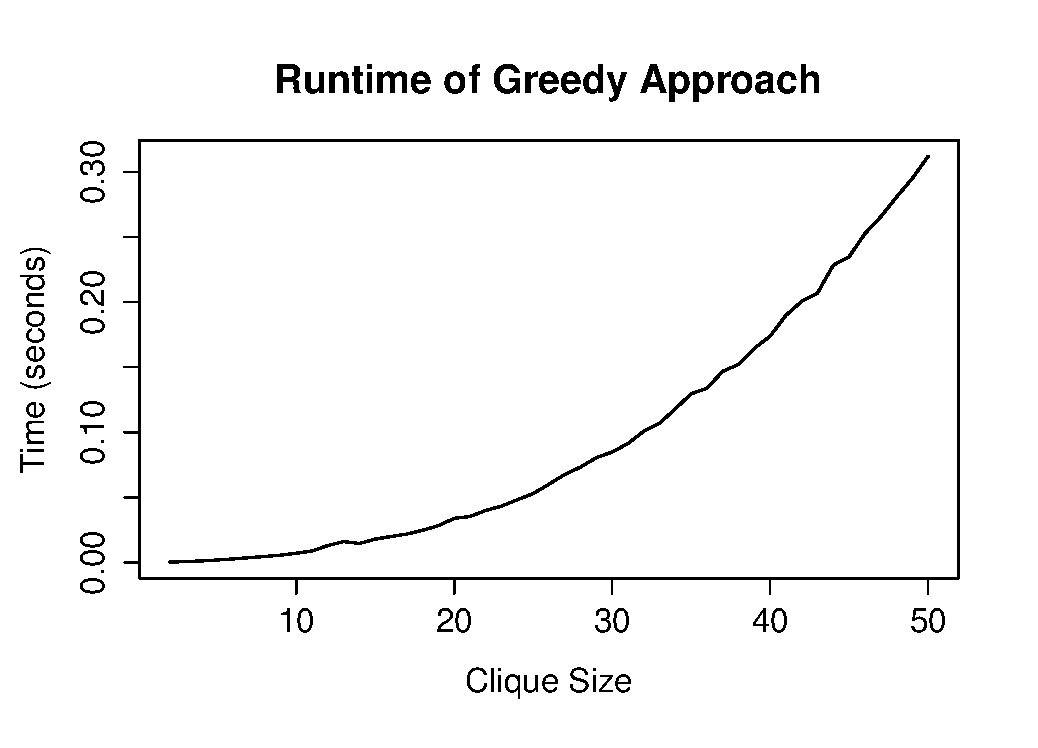
\includegraphics[width=\linewidth]{figures/greedy-runtime}
\caption{Runtime performance of the greedy approach on Cliques sizes from $N=2$ to $N=50$.}
\label{fig:greedy-runtime}
\end{subfigure}\hspace*{\fill}
\begin{subfigure}{0.48\textwidth}
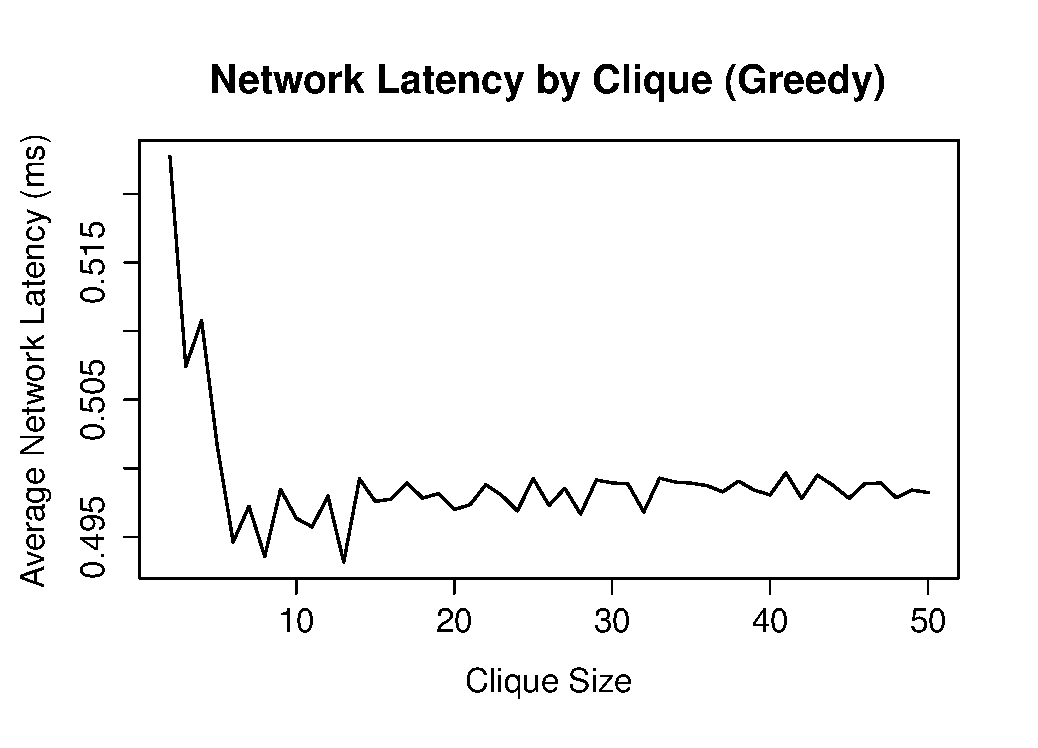
\includegraphics[width=\linewidth]{figures/greedy-latency}
\caption{Average latency of networks formed from the greedy approach on Cliques sizes from $N=2$ to $N=50$.}
\label{fig:greedy-latency}
\end{subfigure}
\end{figure*}


\medskip
\begin{figure*}[ht]
\begin{subfigure}{0.48\textwidth}
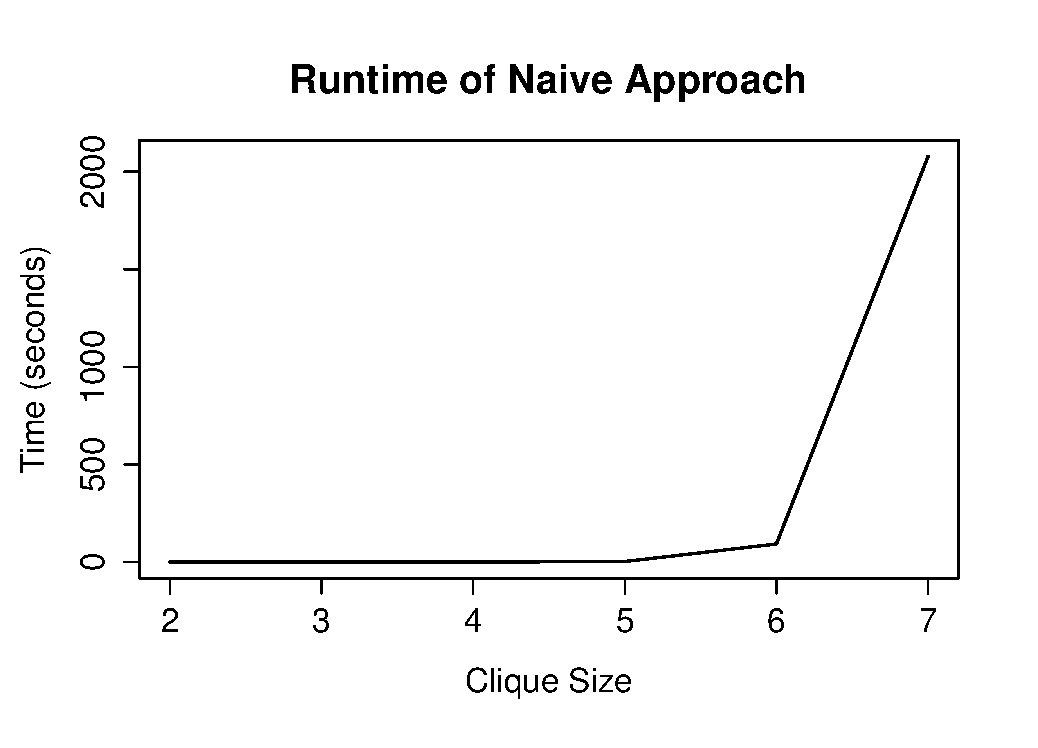
\includegraphics[width=\linewidth]{figures/naive-runtime}
\caption{Runtime performance of the naive approach on Cliques sizes from $N=2$ to $N=7$.}
\label{fig:naive-runtime}
\end{subfigure}\hspace*{\fill}
\begin{subfigure}{0.48\textwidth}
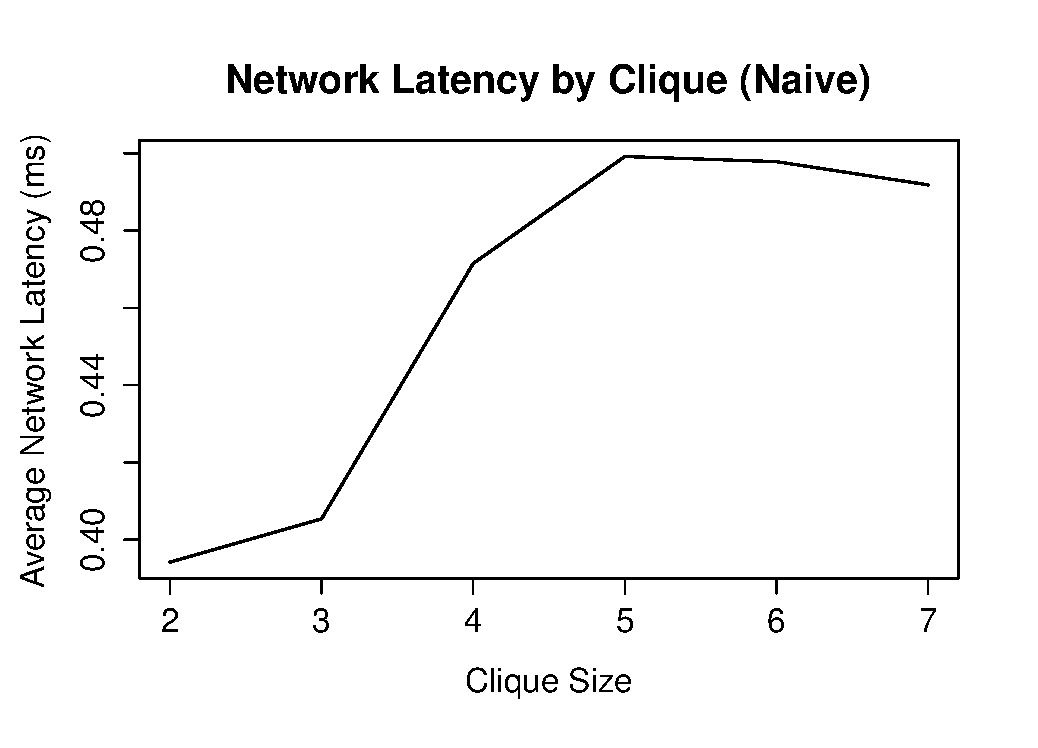
\includegraphics[width=\linewidth]{figures/naive-latency}
\caption{Average latency of networks formed from the naive approach on Cliques sizes from $N=2$ to $N=7$.}
\label{fig:naive-latency}
\end{subfigure}
\end{figure*}

\medskip
\begin{figure*}[ht]
\begin{subfigure}{0.48\textwidth}
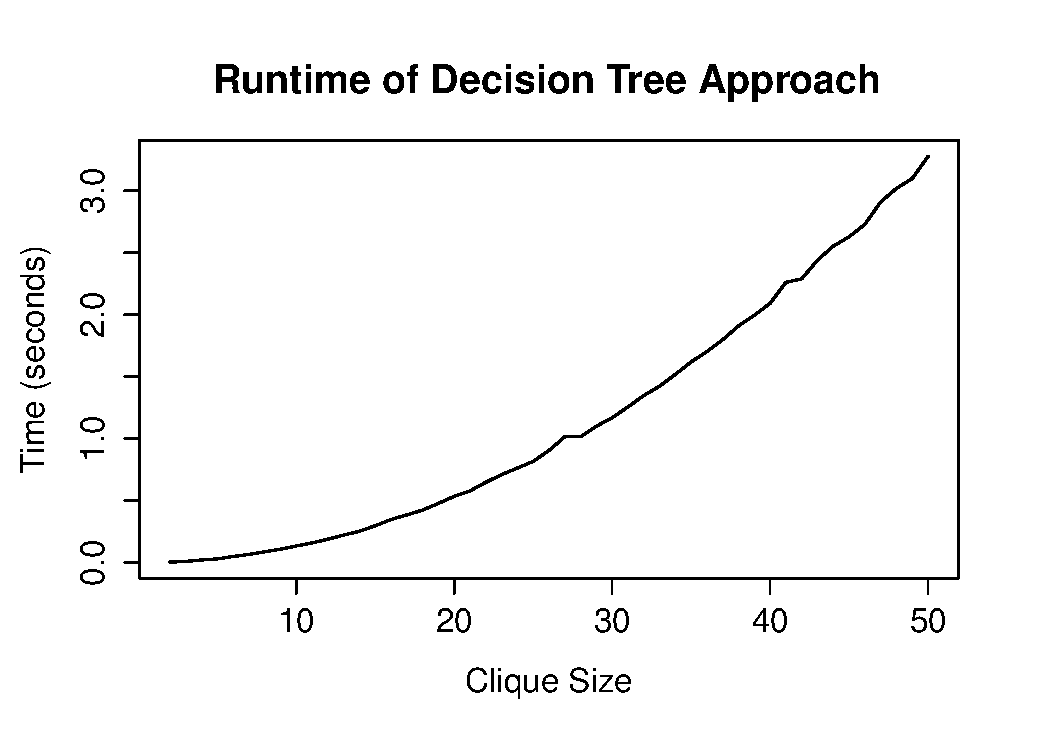
\includegraphics[width=\linewidth]{figures/decisiontree-runtime}
\caption{Runtime performance of the decision tree approach on Cliques sizes from $N=2$ to $N=50$.}
\label{fig:decisiontree-runtime}
\end{subfigure}\hspace*{\fill}
\begin{subfigure}{0.48\textwidth}
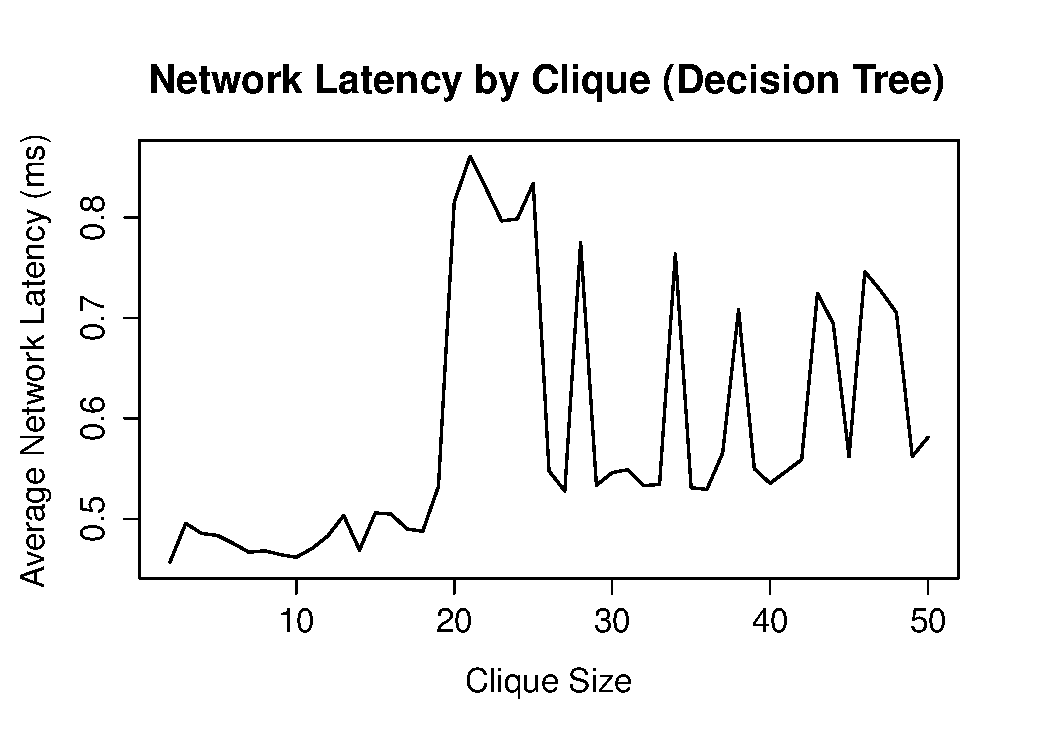
\includegraphics[width=\linewidth]{figures/decisiontree-latency}
\caption{Average latency of networks formed from the decision tree approach on Cliques sizes from $N=2$ to $N=50$.}
\label{fig:decisiontree-latency}
\end{subfigure}
\caption{ Hey John! Please write a comprehensive caption for this set of graphs here} \label{fig:1}
\end{figure*}


%\begin{figure*}[ht]
%  \centering 
%  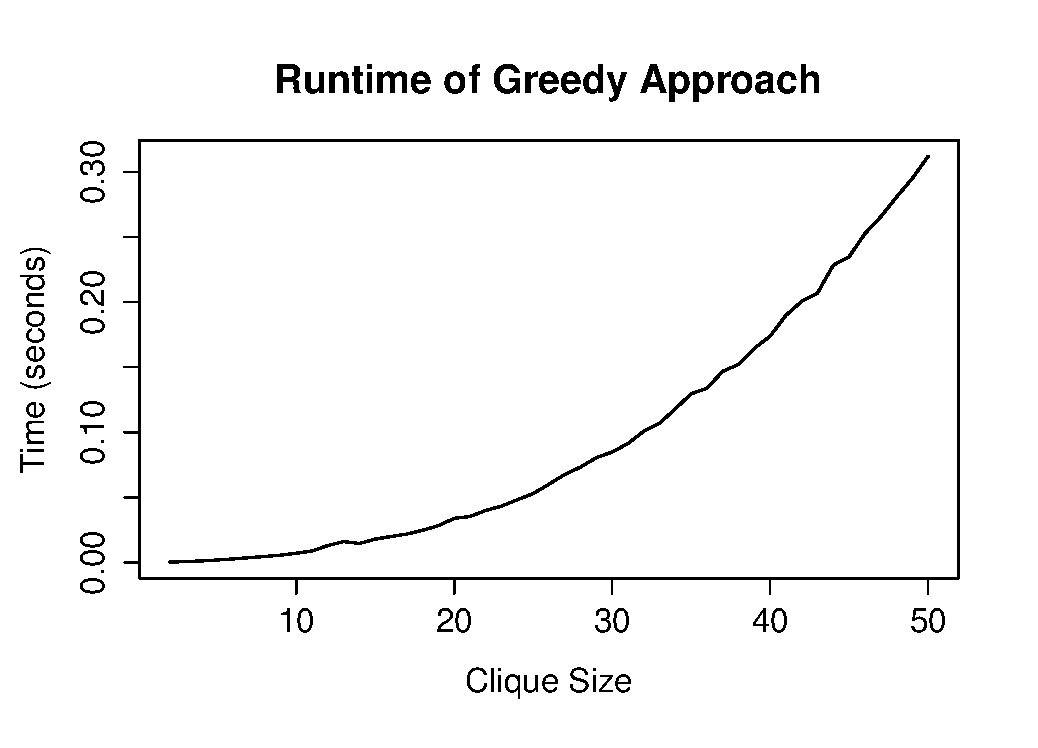
\includegraphics[scale=.8]{figures/greedy-runtime}
%  \caption{Runtime performance of the greedy approach on Cliques sizes from $N=2$ to $N=50$.}
%  \label{fig:greedy-runtime}
%\end{figure*}
%
%
%\begin{figure*}[ht]
%  \centering
%  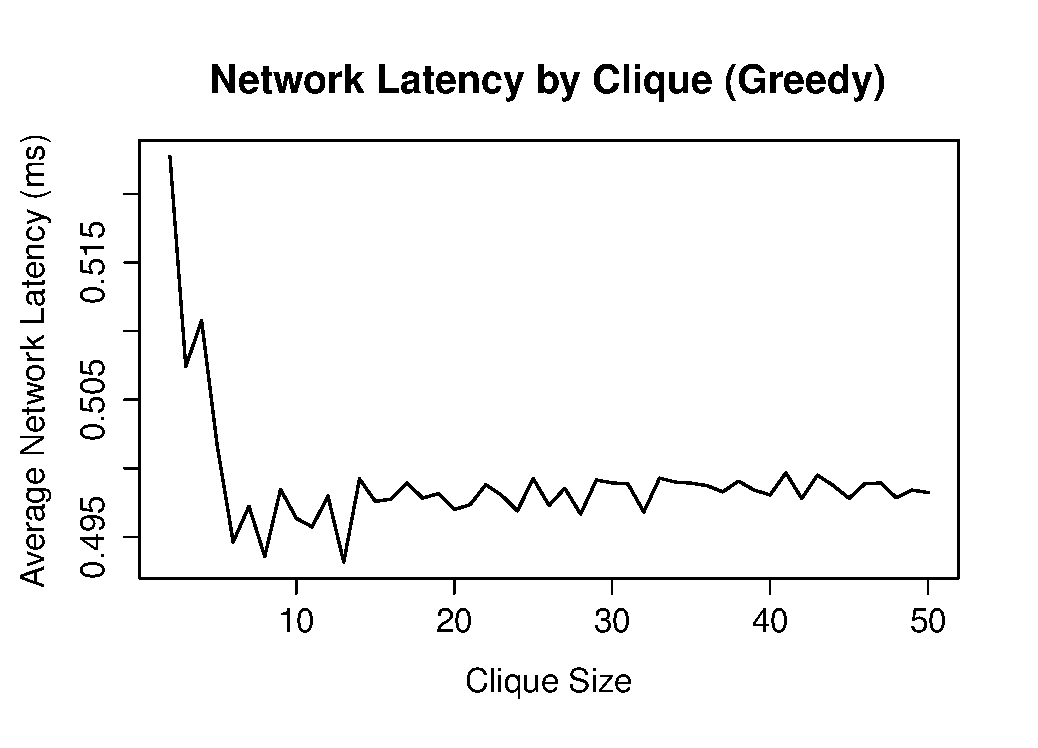
\includegraphics[scale=.8]{figures/greedy-latency}
%  \caption{Average latency of networks formed from the greedy approach on Cliques sizes from $N=2$ to $N=50$.}
%  \label{fig:greedy-latency}
%\end{figure*}
%
%\begin{figure*}[ht]
%  \centering 
%  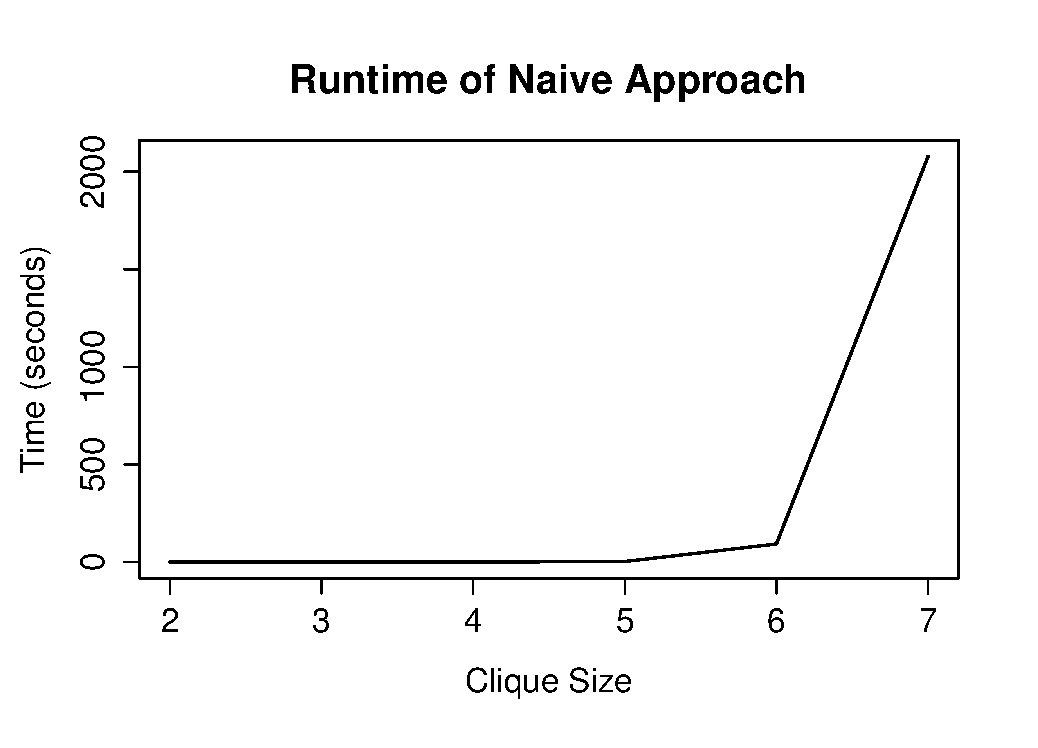
\includegraphics[scale=.8]{figures/naive-runtime}
%  \caption{Runtime performance of the naive approach on Cliques sizes from $N=2$ to $N=7$.}
%  \label{fig:naive-runtime}
%\end{figure*}
%
%
%\begin{figure*}[ht]
%  \centering
%  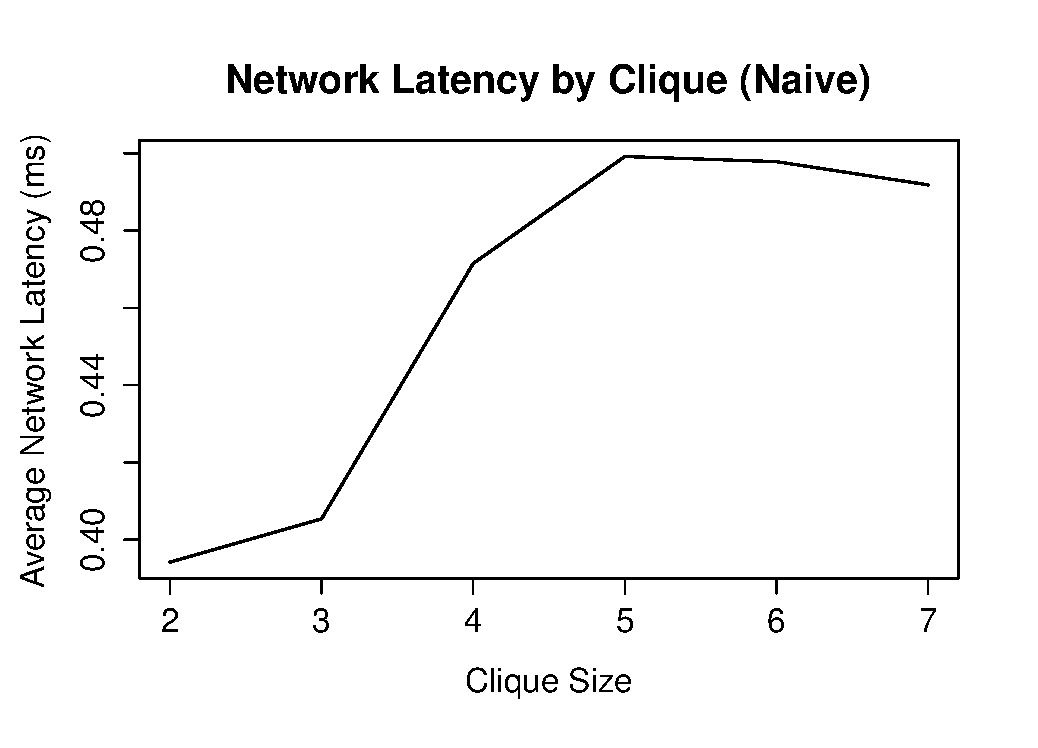
\includegraphics[scale=.8]{figures/naive-latency}
%  \caption{Average latency of networks formed from the naive approach on Cliques sizes from $N=2$ to $N=7$.}
%  \label{fig:naive-latency}
%\end{figure*}
%
%
%
%\begin{figure*}[ht]
%  \centering 
%  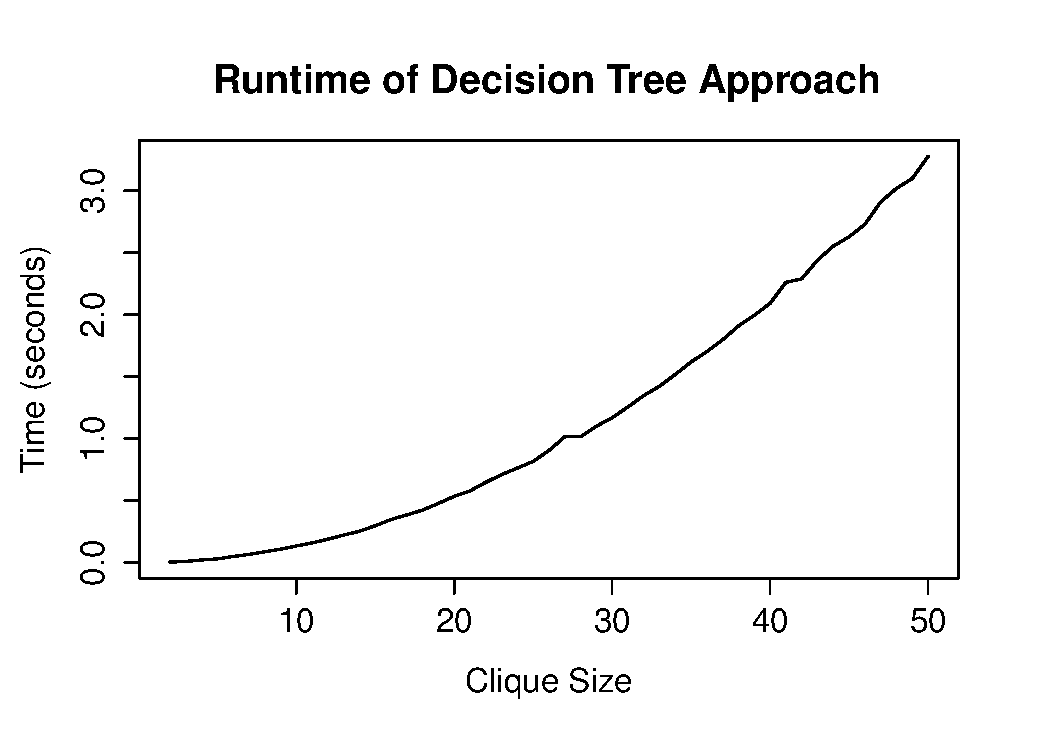
\includegraphics[scale=.8]{figures/decisiontree-runtime}
%  \caption{Runtime performance of the decision tree approach on Cliques sizes from $N=2$ to $N=50$.}
%  \label{fig:decisiontree-runtime}
%\end{figure*}
%
%
%\begin{figure*}[ht]
%  \centering
%  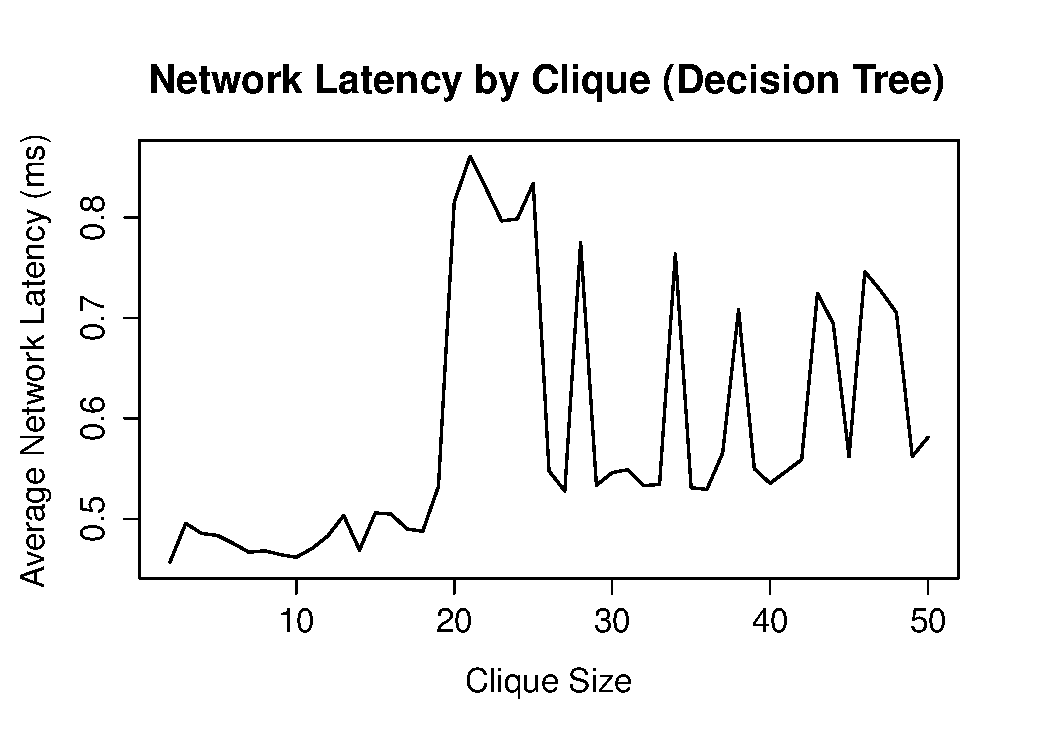
\includegraphics[scale=.8]{figures/decisiontree-latency}
%  \caption{Average latency of networks formed from the decision tree approach on Cliques sizes from $N=2$ to $N=50$.}
%  \label{fig:decisiontree-latency}
%\end{figure*}


%%% Local Variables:
%%% mode: latex
%%% TeX-master: "IPDPS2017"
%%% End:  
\subsection{Related work}
\label{sec:relatedWork}
High scalability and distribution feature are the most important requirements for processing large volume of data which is mostly created by human or connected devices. Cloud computing which is extensively used for data processing, meets both requirements. Although easy launch of instances through web-based console is alluring option, cloud computing brings in series of new challenges as well as security risks, Shared access to the physical resources, availability and consistent performance of applications. Some of the studies on cloud computing focus on {\it performance concern} caused by sharing physical infrastructure among multiple virtual machines.The performance and efficiency of data-driven application have been studied extensively in the literature \cite{hacigumus2002providing, curino2011relational, cooper2010benchmarking}. Techniques to improve workload balancing between clients and server and graph-based partitioning algorithm for improving the performance and obtaining almost linear elastic scale-out is introduced in \cite{curino2011relational}. Furthermore, a new benchmark framework has been established in \cite{cooper2010benchmarking} to compare performance of cloud services offering by various CSPs.

To protect sensitive data from untrusted CSP, most researches focused on {\it Homomorphic Encryption} that allows computations to be carried out over encrypted data \cite{gentry2009fully}. Other crypto-system that relaxed on security notion is Order-Preserving Encryption (OPE) also introduced in \cite{boldyreva2009order} and implemented in \cite{ahmadian2014security,ahmadian2015security} for cloud platform. 

The reported research in this papers, leverages the performance of cluster of cloud instances collaborating in a total system. Ultimate goal is minimizing the latency of allocated instances in the public cloud without enforcing extra cost to the owners with holistic and efficient solution.

\section{Future Work} \label{sec:futurework}

In our experiments we did not determine if the latency observations we made would  translate into stable, low-latency networks for long term usage, i.e., if we identify a low-latency network, how likely is that network to remain low-latency? This question is especially important given the variability of network performance under various loads. In this work we did not address that question but instead hope to address it in future work. 

\section{Conclusion} \label{sec:conclusion}
In this paper we presented a novel method for optimizing networks in the cloud. We presented three different approaches: the naive approach, the greedy approach, and an approach driven by decision tree learning.

In our study we found that for small networks with less than 7 nodes, the most optimal values can be found very quickly using the naive approach. Many networks, however, are not this small. For networks larger than 7, the greedy approach has the best performance while still being able to find networks that satisfy the constraints we examined in this paper. However, if finding the best possible networks is desirable (over runtime complexity) we found that our decision tree approach outperformed the greedy approach with only a minor
increase in runtime performance.

\section{Acknowledgments} \label{sec:acknowledgments}
The work of Leavens and Singleton was supported in part by NSF grants CCF0916350 and CNS1228695. The work of Leavens was also supported by NSF grants CCF0916715 and CCF1017262.


%%% Local Variables:
%%% mode: latex
%%% TeX-master: "IPDPS2017"
%%% End: 

\bibliographystyle{IEEEtran}
\bibliography{report}

% that's all folks
\end{document}
